\ifspanish

\else

Let ${X_k, k \ge 0}$ be a Markov chain with state space ${\cal Z} = \{0, 1, 2, 3\}$. The initial state is 0, that is, $P\{X_0=0\}=1$. If, at time $n$, the process is in state $i<3$, at time $n+1$ it will remain in the same state with probability $1-p$ or jump to state $i+1$ with probability $p$. 
\begin{align*}
P\{X_{n+1}=i+1 \mid X_n=i\} = p   \\
P\{X_{n+1}=i \mid X_n=i\} = 1-p
\end{align*}
If the process is in state 3, it will remain in the same state with probability 1.

\begin{parts}
\part Find the transition matrix
\part Show the transition graph
\part Compute $P\{X_2 = 1 \}$
\part Compute $P\{X_n = 0\}$, for any $n>0$
%\part Compute $P\{X_n = 3\}$, for any $n>0$
\part Find a stationary distribution for this process
\end{parts}

%%%%%%%%%%%%%%%%
\begin{solution}
\begin{parts}

\part
\begin{align*}
{\bf P} = 
	\begin{pmatrix}
	1-p & p   & 0   & 0   \\
	0   & 1-p & p   & 0   \\
	0   & 0   & 1-p & p   \\
	0   & 0   & 0   & 1 
	\end{pmatrix}
\end{align*}

\part
.
\begin{center}
\centering
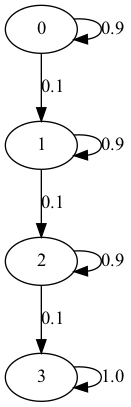
\includegraphics[width=0.1\textwidth]{./db/figs/P202306_markov_chain.png}
\end{center}

\part 
\begin{align*}
P\{X_2=1\} 
   &= \begin{pmatrix} 0 & 1 & 0 & 0 \end{pmatrix}
	  {\bf q}_2
    = \begin{pmatrix} 0 & 1 & 0 & 0\end{pmatrix}
	  {\bf P}^\intercal
	  {\bf P}^\intercal
	  \begin{pmatrix} 1 \\ 0 \\ 0 \\ 0 	\end{pmatrix}   \\
   &= \begin{pmatrix} p & 1-p & 0 & 0\end{pmatrix}
	  \begin{pmatrix} 1-p \\ p \\ 0 \\ 0 	\end{pmatrix}  
    = 2p (1-p) 
\end{align*}

\part $X_n=0$ if and only if there are no transitions from 0 to 1, that is $X_0=X_1=\ldots =X_n=1$. This will happen with probability
\begin{align*}
P\{X_n=0\} = (1-p)^n
\end{align*}
 
\part Eventually, the process will reach state 3 and remain there. Thus $\boldsymbol{\pi}=(0,0,0,1)$ must be a stationary distribution. Indeed,
\begin{align*}
{\bf P}^\intercal \boldsymbol{\pi} = 
	\begin{pmatrix}
	0   \\
	0   \\
	0   \\
	1 
	\end{pmatrix}
	= \boldsymbol{\pi}
\end{align*}


\end{parts}
\end{solution}


\fi